\section{ImageNet Dataset}
\begin{frame}{}
    \LARGE CNN Datasets: \textbf{ImageNet}
\end{frame}

\begin{frame}{ImageNet}
    \begin{itemize}
        \item The most extensive dataset for image classification
        \item 3 RGB channels from 0 to 255
        \item Full ImageNet: 14,197,122 images across 21,841 categories
        \item ILSVRC benchmark subset (used by the architectures in this lecture): 1000 classes, about 1.28M training images
    \end{itemize}

    \begin{figure}
        \centering
        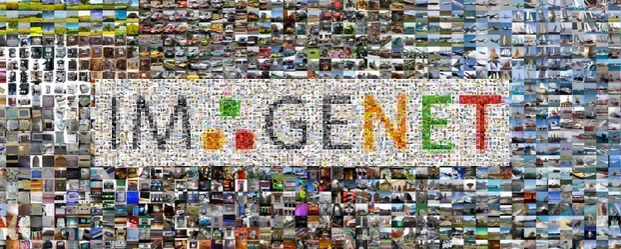
\includegraphics[width=1.0\textwidth,height=0.45\textheight,keepaspectratio]{images/cnn/imagenet.png}
        \caption*{\scriptsize Mosaic of ImageNet sample images; original source unidentified.}
    \end{figure}
\end{frame}

\begin{frame}{ILSVRC Winners}
    \begin{figure}
        \centering
        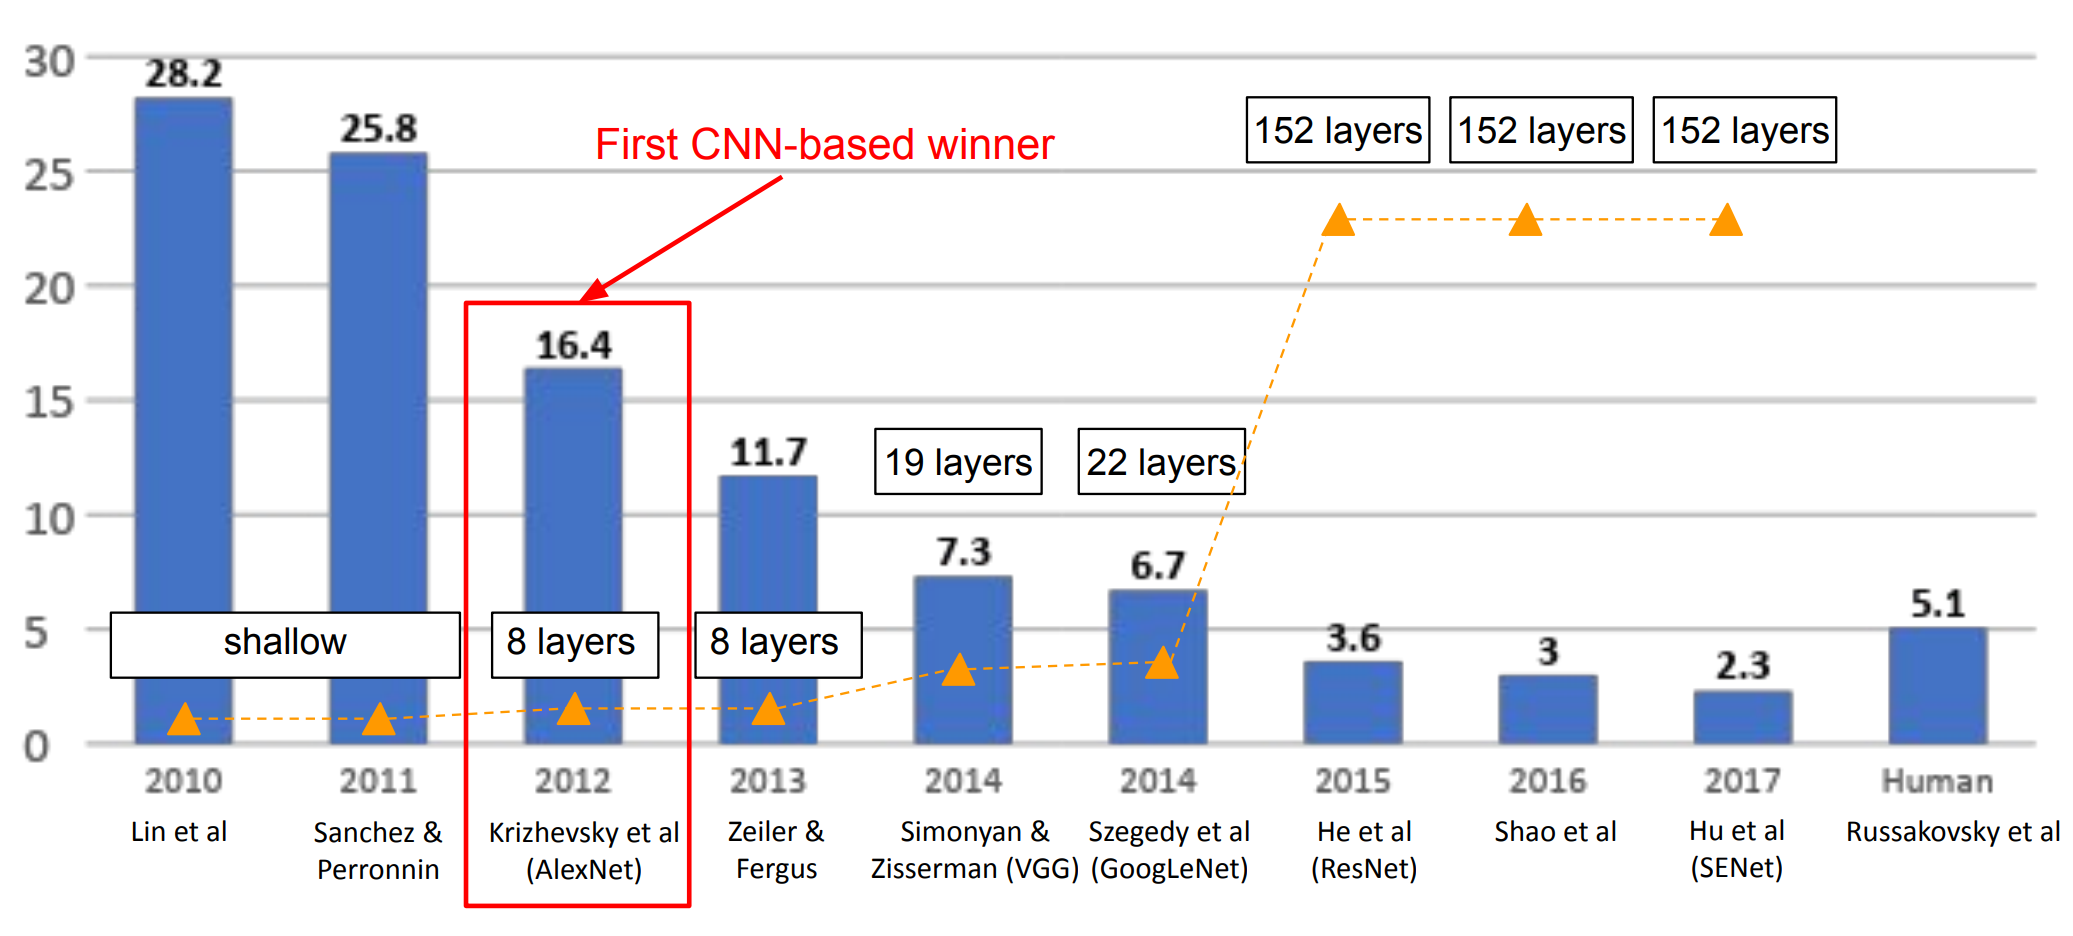
\includegraphics[width=0.95\textwidth,height=1.0\textheight,keepaspectratio]{images/cnn/imagenet_2.png}
        \caption*{\scriptsize Winning top-5 classification error by year. Figure: Stanford CS231n; data from the official ILSVRC results (image-net.org).}
    \end{figure}
\end{frame}